\chapter{Simulations}
\label{chap:simulation}
To illustrate the working principle of IDI and to examine the Signal-to-Noise  characteristics, different simulations were performed:

First, it was assumed that the object to be imaged consists of discrete emitters, each emitting monochromatic spherical waves with the same wavelength, but with a randomly chosen phase, and the speckle image on a pixelated detector was simulated by addition of the scalar electric fields and taking the squared magnitude for each pixel. To reduce the influence of this discrete sampling on the simulated speckle patterns, the simulation is performed at XX the resolution and downsampled, such that each data point is the result of 4x4 discrete calculations
In this configuration, the speckle images of a single particle with randomly positioned emitters inside (approximating a single particle imaging setup), a focal volume filled with randomly positioned (non intersecting) hard spheres consisting of randomly positioned atoms (approximating for example many spherical nano particles imaged simultaneously) as well as a crystalline structure with emitters positioned at within a lattice were simulated. In the first two cases, a small-angle regime was chosen and the reconstruction was performed in 2D and as a 1D radial profile. For the crystalline structure, a realistic lattice constant in the same order of magnitude as the K$\alpha$ wavelength moves the reconstruction out of the small-angle regime and a 3D reconstruction of the reciprocal space was performed.
Additionally, in these simulations the effect of under-sampling was studied.

Second, to examine the influence of the fluorescence lifetime and pulse width, a time-resolved simulation was performed.
The results were compared with the approximation, that the contrast is determined by the product of the different number of modes.

Ultimately, the results of these simulations were used the determine the feasibility of an experimental setup using IDI




\paragraph{Detector effects}
To simulate the influence of detector charecteristics charge-sharing and readout noise, an image degradation is performed: After Poisson sampling the simulated speckle image, for each photon an uniform random position within its pixel is chosen as the center of Gaussian distribution with FWHM of 0.15 pixel  (similar to the size of the PSF for MPCCD detectors XXX).
The intensity within one pixel is given by the integral over the Gaussian,
\begin{equation}
I(\Delta x,\Delta y)=\frac{1}{4} \left(\text{erf}\left(\frac{\sfrac{1}{2}-\Delta x}{\sqrt{2}
	\sigma}\right)+\text{erf}\left(\frac{\sfrac{1}{2}+\Delta x}{\sqrt{2} \sigma}\right)\right) \left(\text{erf}\left(\frac{\sfrac{1}{2}-\Delta y}{\sqrt{2}
	\sigma}\right)+\text{erf}\left(\frac{\sfrac{1}{2}+\Delta y}{\sqrt{2} \sigma}\right)\right)
\end{equation}
with $\sigma$ the standard deviation of the Gaussian in pixels and $\Delta x$, $\Delta y$ the distance of the pixel to the chosen photon center, and evaluated for the neighboring pixels. Afterwards a Gaussian readout noise is added. The effect of this degradation on the spectrum is illustrated in \fref{fig:degrad}.


\begin{figure}
	\centering
\includegraphics[width=0.8\linewidth]{images/sharing.png}
	\caption[Effect of charge sharing and detector noise]{Effect of charge sharing and detector noise on the spectrum of the simulated speckle pattern.}
	\label{fig:degrad}
\end{figure}



\section{Time independent Simulations}
In an infinite coherence time, stationary sources approximation, the simulation of the speckle pattern can be performed time independently the superposition of scaler electrical fields emitted with random phases. The simulation of the intensity at multiple discrete points can be performed in parallel using GPU acceleration, resulting in a simple and fast to evaluate model.



- Reconstruction shape
- Dependence in Nimages, Dependence on Npairs, dependence on modes, random orientations





\subsection{Reconstruction}

\paragraph{Photon counting}
As the relevant signal for the correlation analysis is the presence of fluorescence photons, but charge sharing and readout noise of the detector as well as the presence of photons caused by air scattering degrades this signal, different approaches  of preprocessing will be compared:

\begin{itemize}
	\item Using the raw signal
	\item Using the raw signal after applying a threshold.
	\item Discretization by closest number of signal photons
	\item Discretization by closest possible combination for each pixel
	\item Discretization by maximum likelihood
	\item Droplet algorithm
\end{itemize}
The noise thresholding will be done with a threshold of 3$\sigma$. To find the closest number of signal photons, the signal after thresholding is divided by the expected energy of a single photon and rounded to the closest integer. Considering possible combinations of signal and scattering photons by finding  $nE_{fluorescence}+mE_{excitation}$ with integer $n$, $m$ closest to the observed value and only using the signal photon number $n$ for the correlation would suppress the influence of scattering, but would still be influenced by charge sharing and doesn't account for the different probabilities of signal and scattering photons.

If the detector noise level, the PSF due to charge sharing as well as the distribution of signal and scattering is known, a Bayesian classifier can be trained on synthetic data, which each observed value on the detector, returns the number of signal photons with the highest conditional probability (\fref{fig:probs}). Depending on the apriori probabilities and the detector characteristics, this maximum likelihood solution can differ from the closest combination. If those parameters are not known with reasonable certainty, an educated guess can still provide decision boundaries.

\begin{figure}
	\centering
	\begin{subfigure}[b]{0.45\textwidth}
		\includegraphics[width=\linewidth]{images/hist.pdf}
		\caption{Histogram}
	\end{subfigure}
	\begin{subfigure}[b]{0.45\textwidth}
		\includegraphics[width=\linewidth]{images/probs.pdf}
		\caption{Probabilities and Decision Boundaries}
	\end{subfigure}
	\label{fig:probs}
	\caption[Histogram, probabilities and decision boundaries for the photon number]{For a Poisson distributed signal with mean 0.01 photons/pixel, a Poisson distributed scattering with mean 0.001 photons/pixel and an photon energy of 1.3 times the energy of a signal photon, a charge sharing PSF with $\sigma$ 0.1 pixel and a Gaussian noise with $\sigma$ 0.05 photons, the simulated histogram is shown on the left. The probabilities of an observed energy being caused by a certain number of signal photons is shown on the right, the dashed lines mark the decision boundaries for an Bayesian classifier.} 
\end{figure}
For comparison, the PSANA Photon algorithm, a droplet algorithm considering only the signal photons is used \ref{psana}.

Possible avenues for improvement would be to use a more sophisticated droplet scheme based on error minimization allowing for subpixel resolution, incorporating the scattering photons into the droplet algorithm or using a neural network trained on synthetic images.




\paragraph{Normalisation}
Mean of all pixels 
Mean of all pixels inside the overlap

If only a single image is taken, the expectation value for each pixel has to be approximated.

If multiple images are taken, under the assumption of ergodicity, the expectation value for each pixel can be approximated by its mean over many images. To account for fluctuations in the exciting FEL pulse and resulting fluctations of the fluorescence intensity, it can be assumed that the distribution over pixel  intensities and FEL intensities are uncorrelated, and the detection probability of each pixel in each shot can be factorized into the product of the probability to detect a photon in a pixel and to detect a photon in a shot. Therefor, the effect of the FEL intensity fluctuations can be suppressed by normalizing each image by the total intensity of the image.
\subsection{Single Sphere}
radial symmetrie

\subsection{Multiple Spheres}


\subsection{Crystal}


\subsection{Superlattice}

\section{Time dependent Simulations}

Each of the $N$ atoms is assigned an emitting time $t_{n}$ chosen according to the excitation pulse shape and its position. Starting from this emitting time, the atom emits an exponential decaying field with a decay time chosen to match the lifetime. 



For each discrete pixel on the simulated detector, for each atom the distance $d_n$, the arrival time $t'_n=t_n+d_n/c$ of each atom's initial radiance, and its time independent complex field $E_n=\frac{1}{d} e^{ikd_n+\phi_n}$ with initial random phase $phi$ is calculated.
The time dependent E field is the summation over the decaying field of all atoms,
\begin{equation}
E(t)=\sum_{n=1}^N  E_n \Theta(t'_n  - t) * e^{-(t-t'_n )/\tau}
\label{eq:tdsum}
\end{equation}
and the simulated intensity the time integral over the magnitude squared of the E-field,
\begin{equation}
I=\int_0^\infty \left| E(t) \right|^2 .
\label{eq:tdint}
\end{equation}

To efficiently solve this integral for each detector pixel, it can be split into N parts with a constant number atoms which radiations have already arrived, and each of those parts can be solved analytically. For this, first all atoms are sorted by the arrival time at the pixel. At each arrival time $t'_n$, the sum in \fref{eq:tdsum} gets a new term and the field is calculated as
\begin{equation}
E(t_n)=E(t_{n-1})*e^{\sfrac{t_{n-1}-t_n}{\tau}}+E_n
\end{equation}
 This can be done with a parallel inclusive scan, as shown in \fref{algo:td}. This gives the supports for the integral, as show in \fref{fig:tdplot}, which can now be solved as
\begin{align}
	I&=\int_0^\infty \left| E(t) \right|^2 = \sum_{n=1}^{N-1} \int_0^{t_{n+1}-t_n} \left|E(t_n)\right|^2 e^{-2t/\tau} \dif t +\int_0^\infty \left| E(t_N)\right|^2 e^{-2t/\tau} \dif t \\
	 &=  \frac{\tau}{2}  \left|E(t_N)\right|^2 -  \frac{\tau}{2}\sum_{n=1}^{N-1} \left|E(t_n)\right|^2 (e^{-2 (t_{n+1}-t_n)/\tau} -1 ) 
\end{align}

This procedure is efficient in regards of discrete time steps that need to be calculated and can easily be run on a GPU.

In \fref{fig:tdpshere} the results of a simulation with Gaussian pulses with different for a single spherical object is shown. The dependence of the speckle visibility and the visibility of the reconstructions is in agreement with the theoretical considerations.

To investigate the influence of sample thickness for crystalline samples as second simulation is performed. As a thicker sample gives more photons and therefore less Poisson noise, but a higher number of temporal and spatial modes and therefore a lower expected lower speckle visibility, a simulation close to experimentally feasible parameters is desirable.



\begin{figure}
	   \centering
		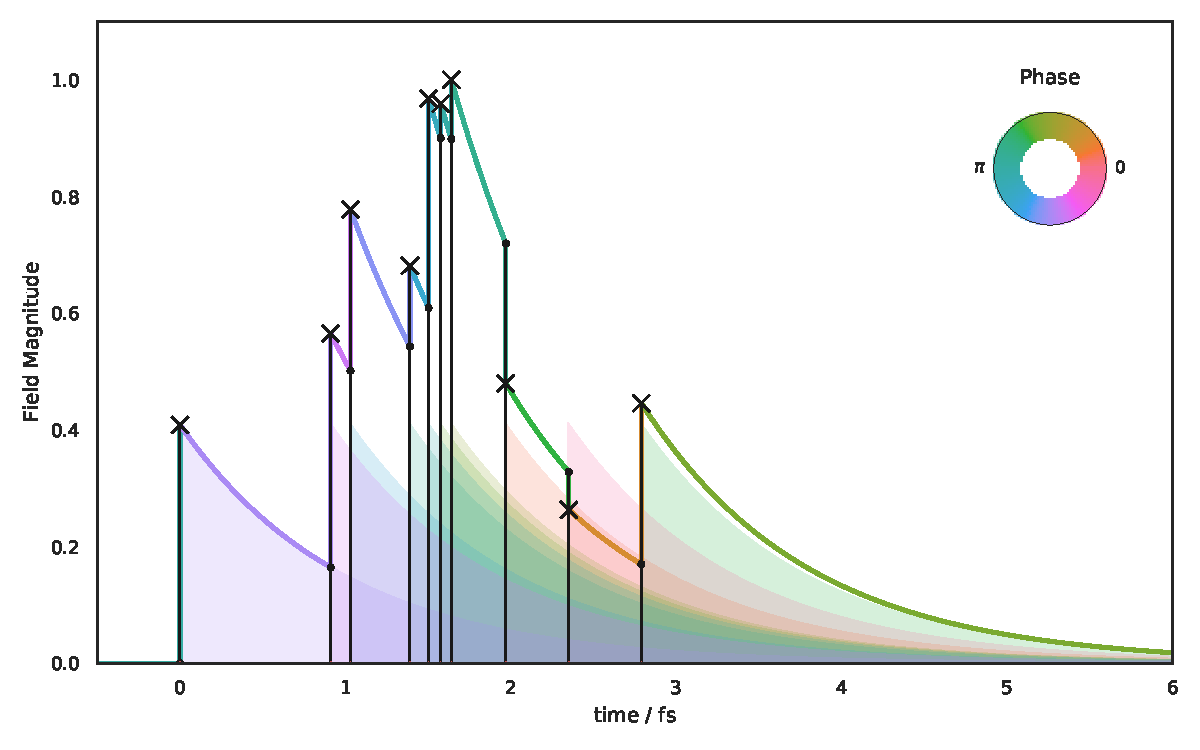
\includegraphics[width=0.7\linewidth]{images/tdplot.pdf}
	\caption[Integration in Time Dependent IDI Simulation]{To illustrate the integration in the time dependent IDI simulation, the (normalized) scalar field at one point of the detector created by 10 emitting atoms with $\tau$=1\,fs and a pulse FWHM of 2\,fs is shown. The solid colors show each atom's field, the line plot the (phase correct) sum. The simplify the calculations, only the time points marked with stars are calculated. To solve the integral \fref{eq:tdint}, it's sufficient to calculated the squared magnitude at those points and to do a piecewise integration from each star-shaped marker the next dot-shaped marker. The color wheel in the top right shows colors used for phase encoding in the plot.}
	\label{fig:tdplot}
\end{figure}


\begin{figure}
	\begin{subfigure}[b]{0.45\textwidth}
		\includegraphics[width=\linewidth]{images/timedependent_1.pdf}
		\caption{Speckle SNR for different pulse FWHM and decay times $\tau$}
	\end{subfigure}
	\begin{subfigure}[b]{0.45\textwidth}
		\includegraphics[width=\linewidth]{images/tdsphere.pdf}
		\caption{Reconstructed radial profiles at different pulse FWHM and fixed decay time $\tau = 0.1$\,fs}
	\end{subfigure}

	\begin{subfigure}[b]{0.45\textwidth}
		\includegraphics[width=\linewidth]{images/timedependent_2.pdf}
		\caption{Visibility of the reconstruction for different pulse FWHM and decay times $\tau$}
	\end{subfigure}
	\caption[Time Dependent IDI Simulation of a Sphere]{Time Dependent IDI Simulation of a Sphere: For a sphere with 10\,nm radius consisting of $2*10^5$ atoms emitting 6.4\,keV fluorescence captured by an 256x256@50\,um detector in 20\,cm distance, a series of simulations were performed with different decay times $\tau$ of the emission and different exciting pulse FWHM. In a) the SNR of the simulated speckle pattern is compared with the theoretical  $1/\sqrt{erfcx(2\sigma/\tau}$ dependence on the ratio of pulse length and $\tau$. In b) exemplary radial profiles of the reconstruction of 50 images each are shown for one fixed $\tau$. Those reconstructions are used to plot the  dependence of the visibility on the pulse width in c). For long pulses, the reciprocal dependence on the pulse length is visible.}
	\label{fig:tdpshere}
\end{figure}



\section{Implications for an experimental design}

